%+----------------------------------------------------------------------------+
%| SLIDES: PostDoc interview presentation
%| Duration: 20 minutes
%| Contents: 7 slides
%|					 (extimated duration 3 minutes per slide )
%| Author: Antonio miti
%| Place: Bonn, January 2022
%+----------------------------------------------------------------------------+



\documentclass[10pt]{beamer}

	
%- Packages ----------------------------------------------------------------------------------------------
\usepackage{../custom-style}



%--Beamer Style-----------------------------------------------------------------------------------------------
\usetheme{toninus}

%- Macros -------------------------------------------------------------------------------------------
\providecommand{\vHam}{\mathscr{v}}
\renewcommand{\checkpoint}[0]{
	\setcounter{tocdepth}{1}
	\addtocounter{framenumber}{-1}
 	\begin{frame}[t]{Outline}
  		%\tableofcontents[currentsection,currentsubsection]
  		%
  		\tableofcontents[currentsection]
		%
	\end{frame}
}

\newcommand{\smark}{\textcolor{orange}{\ding{43}}}%


%- TEMP -----------------------------------------------------------------------------
\newtcolorbox[auto counter,number within=section]{probox}[2][]{%
	fonttitle= \footnotesize \bfseries,
	title=#2,
	fontupper=\footnotesize,%\sffamily,
	colback=white,
	colbacktitle=white,
	coltitle=orange!70!black,
	colframe=orange!70!black,
	%boxrule=1pt,
	titlerule=0pt,
	toptitle=-0.2em,bottomtitle=-0.2em, %title spacing	
	colback=white,
	leftupper=-3mm,rightupper=0mm,top=0mm,bottom=0mm, 
	#1,
}

\renewcommand{\action}{\curvearrowright}


%- T1tle P4g3 -------------------------------------------------------------------------------------------
\title{Research overview} 
\subtitle{}
\author[AMM]{\href{https://dmf.unicatt.it/miti/}{Antonio Michele Miti}}
\institute[Mpim]{
	\vspace{3em}
	\\
	MPIM, Bonn, Germany 
	\\
	\vspace{.5em}
	\href{https://www.mpim-bonn.mpg.de/}{
\includegraphics[width=6cm]{../Logos/Mpim_logo}}
	\vspace{3em}
}
\date[Mpim_22] % (optional, should be abbreviation of conference name)
{	
	{\vskip 1ex}
	UCSC Interview, February 8, 2022
}


%---------------------------------------------------------------------------------------------------------------------------------------------------
%- D0cum3nt ----------------------------------------------------------------------------------------------------------------------------------
\begin{document}
%------------------------------------------------------------------------------------------------

%-------------------------------------------------------------------------------------------------------------------------------------------------
\maketitle
%-------------------------------------------------------------------------------------------------------------------------------------------------


%-------------------------------------------------------------------------------------------------------------------------------------------------
\section{Research statement: framework \& current results}
\checkpoint
%-------------------------------------------------------------------------------------------------------------------------------------------------



%-------------------------------------------------------------------------------------------------------------------------------------------------
\begin{frame}[t, fragile]{Research Framework:  \textbf{multisymplectic geometry}} %Fragile -->workaround tikzcd
	\begin{center}
		$-$ \emph{multisymplectic means \textbf{going higher} in the degree of $\omega$} $-$
	\end{center}
	\vfill
	\pause
	\begin{defblock}[$n$-plectic manifold ~\emph{(Cantrijn, Ibort, De Le\'on)} \cite{Cantrun2017}]
		\includestandalone[width=0.95\textwidth]{../Pictures/Figure_multisym}	
	\end{defblock}
	%
	\vfill
	%
	%
	\pause
	\begin{block}{Examples:}
		\begin{itemize}
			\item[$\bullet$] 1-plectic $=$ symplectic
			\item[$\bullet$] Any oriented $(n+1)$-dimensional manifold is $n$-plectic w.r.t. the volume form.
			\item[$\bullet$] The multicotangent bundle $\Lambda^n T^\ast Q$ is naturally $n$-plectic.
		\end{itemize}
	\end{block}			 
%
	\pause
	\begin{block}{Historical motivation}
		Mechanics: geometrical foundations of \textit{(first-order)} field theories.
		\begin{itemize}
		 \item[•] Kijowski, W. Tulczyjew \cite{Kijowski1979}; %(1979)
		 \item[•] Cariñena, Crampin, Ibort \cite{Carinena1991b};% (1991)
		 \item[•] Gotay, Isenberg, Marsden, Montgomery \cite{Gimmsy1};%(1998)
		 \\ $\cdots$
		\end{itemize}
	\end{block}
\end{frame}
%-------------------------------------------------------------------------------------------------------------------------------------------------


%-------------------------------------------------------------------------------------------------------------------------------------------------
\begin{frame}{Observables in \textbf{multisymplectic geometry}}
	%
	\begin{defblock}[Hamiltonian $(n-1)$-forms]
		\begin{displaymath}
			\Omega^{n-1}_{ham}(M,\omega) 	:=
			\biggr\{ \sigma \in  \Omega^{n-1}(M) \; \biggr\vert \; 
				\exists \vHam_\sigma \in \mathfrak{X}(M) ~:~ 
				\tikz[baseline,remember picture]{\node[rounded corners,
                        fill=orange!5,draw=orange!30,anchor=base]            
            			(target) {$d \sigma = -\iota_{\vHam_\sigma} \omega$ };
            	}				
				~\biggr\} 
			\end{displaymath}
	\end{defblock}
	%
	\onslide<2>{
		\tikz[overlay,remember picture]
		{
			\node[rounded corners,
                 fill=orange!5,draw=orange!30,anchor=base]
            	 (base) at ($(current page.north east)-(2,1)$) [rotate=-0,text width=3.5cm,align=center] {\footnotesize{\textcolor{red}{Hamilton-DeDonder-Weyl \\equation}}};
		}	
		\begin{tikzpicture}[overlay,remember picture]
		    	\path[->] (base.south east) edge[bend left,red](target.east);
	    \end{tikzpicture}
	}
	%
	\vspace{-1em}
	\pause
	\begin{columns}[T]
		\setlength{\belowdisplayskip}{5pt}
		\begin{column}{.50\linewidth}
			%
			\centering \it
			$-$ symplectic case $-$
			\onslide<3->{
			\begin{thmblock}[Observables Poisson algebra]
				$C^\infty(M,\omega)$ endowed with
				\vspace{-.5em}
				\begin{displaymath}
					\lbrace \sigma_1, \sigma_2 \rbrace =			
					~ - \iota_{\vHam_1}\iota_{\vHam_2} \omega 
					~= \mathcal{L}_{\vHam_1} \sigma_2
				\end{displaymath}			
				forms a Poisson algebra.
			\end{thmblock}
			}
			%
			\onslide<4->{
			\vspace{1em}
			\begin{itemize}
				\item[\cmark] Skew-symmetric;
				\item[\cmark] multiplication of observables;
				\item[\cmark] Leibniz Rule;
				\item[\cmark] Jacobi equation;
			\end{itemize}		
			}		
		\end{column}	
		%
		\onslide<1->{\vrule{}}
		%
		\begin{column}{.50\linewidth}
			\centering \it
			$-$ $n$-plectic case $-$
			\onslide<5->{			
			\begin{thmblock}[Observables $L_\infty$-algebra]
				$\Omega^{n-1}_{ham}(M,\omega)$ endowed with
				\vspace{-.5em}
				\begin{displaymath}
					\lbrace \sigma_1, \sigma_2 \rbrace =			
					~ - \iota_{\vHam_1}\iota_{\vHam_2} \omega 
				\end{displaymath}			
				can be extended to a \\ $L_\infty-algebra$.
			\end{thmblock}
			}
			%
			\onslide<6->{
			\begin{itemize}
				\item[\cmark] Skew-symmetric;
				\item[\xmark] multiplication of observables;
				\item[\xmark] Jacobi equation;
				%\\ \hspace*{4.25em} full-fledged Jacobi equation;
				\item[\smark] Jacobi equation \emph{up to homotopies}.
			\end{itemize}			
			}
		\end{column}	
	\end{columns}
\end{frame}
%-------------------------------------------------------------------------------------------------------------------------------------------------



%-------------------------------------------------------------------------------------------------------------------------------------------------
\begin{frame}[t]{Symmetries in \textbf{multisymplectic geometry}}
	Consider a Lie algebra action $v:\mathfrak{g} \to \mathfrak{X}(M)$  preserving the $n$-plectic form $\omega$,
	\vfill

	\vspace{-1em}
	\begin{columns}[T]
		\setlength{\belowdisplayskip}{5pt}
		\begin{column}{.50\linewidth}
			%
			\centering \it
			\onslide<2->{
				$-$ symplectic case $-$
				\begin{defblock}[Comoment map pertaining to $v$]
					Lie algebra morphism
					$$ f: \mathfrak{g} \to C^\infty(M) $$
					such that
					$$ d~f (x) = -\iota_{v_x} \omega \qquad \forall x \in \mathfrak{g}~.$$
				\end{defblock}
			}
		\end{column}	
		%
		\onslide<2->{\vrule{}}
		%
		\begin{column}{.50\linewidth}
			\centering \it
			\onslide<3->{			
				$-$ $n$-plectic case $-$
				\begin{defblock}[Homotopy comoment map \tiny (HCMM)]
					$L_\infty$-morphism 
					$$ (f_k) : \mathfrak{g} \to L_\infty (M,\omega)$$
					such that
					$$ d~f_1(x) = -\iota_{v_x} \omega \qquad \forall x \in \mathfrak{g}~.$$
				\end{defblock}	
			}
		\end{column}	
	\end{columns}	
	%
	\pause
	\vfill
	\centering 
	\onslide<4->{\textbf{-- Conserved quantities --}}
	%
	\vspace{-.5em}
	\begin{columns}[T]
		\setlength{\belowdisplayskip}{5pt}
		\begin{column}{.50\linewidth}
			%
			\centering \it
			\onslide<4->{
			\begin{propblock}[Noether Theorem]
				\small Fixed $H\in C^\infty_{\text{Ham}}(M)$ ($\mathfrak{g}$-invariant) ,
				$$\mathcal{L}_{v_H} f(x) = 0 \qquad \forall x \in \mathfrak{g}$$
			\end{propblock}
			}
		\end{column}	
		%
		\onslide<5->{\vrule{}}
		%
		\begin{column}{.50\linewidth}
			\centering \it
			\onslide<5->{			
			\begin{propblock}[RWZ16 Theorem]
				\small Fixed $H\in \Omega^{n-1}_{\text{Ham}}(M)$ ($\mathfrak{g}$-invariant),
				$$\mathcal{L}_{v_H} f_k(p) \in B^k(M) \qquad \forall p \in Z_k(\mathfrak{g})$$			
			\end{propblock}
			}
		\end{column}	
	\end{columns}		
\end{frame}
%-------------------------------------------------------------------------------------------------------------------------------------------------





%-------------------------------------------------------------------------------------------------------------------------------------------------
	\begin{frame}{Results}
		\vspace{1em}
		
		\begin{columns}
			\begin{column}[T]{0.3\textwidth}
				\centering
				\onslide<1->{
					\fbox{
\includegraphics[width=.9\textwidth]{../Pictures/cover-JAMS}}
				}
			\end{column}		
			\begin{column}[T]{0.7\textwidth}
				\begin{itemize}
					\item[-] Explicit \emph{Homotopy comomentum map} coming from hydrodynamics ( ideal fluid configurations as Lie algebra action)
					\item[-] Relations with \emph{knot theory} (hydrodinamics interpretation: links as concentrated vortices).
				\end{itemize}
			\end{column}		
		\end{columns}	
		
		\vspace{1em}
		\begin{columns}[T]
			\begin{column}{0.3\textwidth}
				\centering
				\onslide<2->{
					\fbox{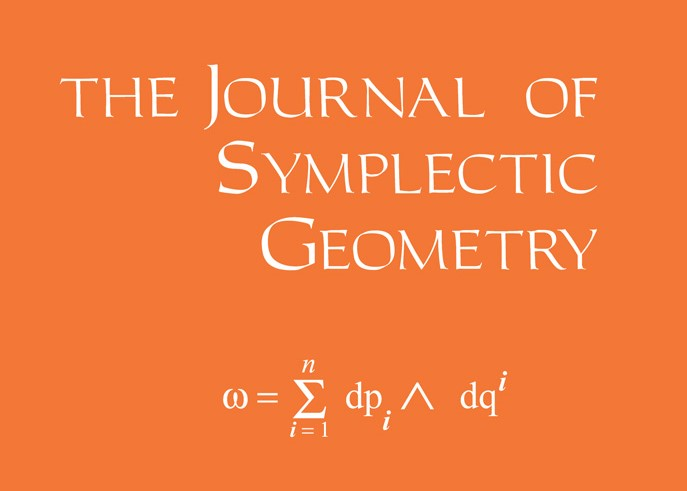
\includegraphics[width=.9\textwidth]{../Pictures/cover-JSG}}
				}
			\end{column}		
			\begin{column}{0.7\textwidth}
				\begin{itemize}
					\item<2->[-] Complete classification of Hamiltonian actions on spheres (multisymplectic w.r.t. the canonical volume form).
					\item<2->[-] Explicit expression of momenta for $SO(n)\circlearrowleft S^n$ and other cases.
				\end{itemize}
			\end{column}		
		\end{columns}		
		
		\vspace{1em}
		\begin{columns}[T]
			\begin{column}{0.3\textwidth}
				\centering
				\onslide<3->{
					\fbox{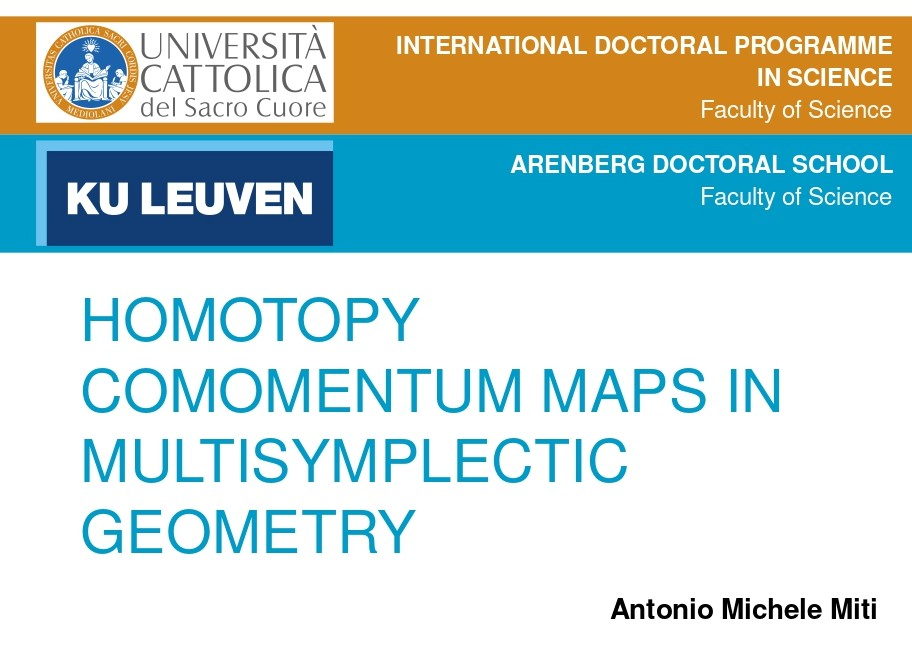
\includegraphics[width=.9\textwidth]{../Pictures/cover-Thesis}}
				}
			\end{column}		
			\begin{column}{0.7\textwidth}
				\begin{itemize}
					\item<3->[-] Compatibility of \emph{Homotopy comomentum maps} w.r.t. gauge-related multisymplectic manifolds.
					\item<3->[-] Relationship between the $L_\infty$-algebra of observables and \emph{higher courant algebroids.} 				
				\end{itemize}	
			\end{column}		
		\end{columns}
		\vfill
\end{frame}
%---------------------------------------------------------------------------------------------------------------------------------------------------


%-------------------------------------------------------------------------------------------------------------------------------------------------
\section{Research proposal: prospective future work}
\checkpoint
%-------------------------------------------------------------------------------------------------------------------------------------------------

%---------------------------------------------------------------------------------------------------------------------------------------------------
\begin{frame}{Research proposal context: (multi)symplectic reduction}
	\textbf{\color{UniGreen}Symplectic reduction:}~~
	Procedure associating to any (suitably regular) pair of symplectic manifold and Hamiltonian action another symplectic manifold of smaller dimension.
	\vfill
	\pause
	\begin{thmblock}[Marsden-Weinstein reduction]
		\vspace{-.4em}
		\begin{tabular}{l p{12cm}}
		    Given: & $(M,\omega)$ symplectic
		    \\
		    & $G\curvearrowright M$ symplectic with equivariant momap. $J:M\to \mathfrak{g}^*$
		    \\[.2em]
		    Assume: & $\mu \in \mathfrak{g}^*$ regular value of $J$ 
		    \qquad\quad \footnotesize \textcolor{gray}{($\Rightarrow$ $J^{-1}(\mu)\hookrightarrow M$ smooth embedding)}
		    \\
			& $G_\mu\action J^{-1}(\mu)$ free and proper
			\quad \footnotesize \textcolor{gray}{($\Rightarrow$ $J^{-1}(\mu)/G_\mu$ smooth manifold)}
			\\[.4em]
			Then: & $\exists!$ symplectic structure $\omega_\mu$ in $M_\mu:= J^{-1}(\mu)/G_\mu$ \\
			& s.t. $\pi^\ast \omega_\mu = j^\ast \omega$ with $j:M_\mu \hookrightarrow M$ and $\pi:M\twoheadrightarrow M_\mu$
		\end{tabular}
		\vspace{-.4em}
	\end{thmblock}
	%
	\vfill
	\pause
	\begin{columns}
		\begin{column}{0.40\textwidth}
			\includegraphics[width=\textwidth]{../Pictures/LessigReduction-pic}
		\end{column}	
		
		\begin{column}{0.6\textwidth}
				\textbf{\color{UniGreen}In mechanics:}~~
			it embodies the process of restricting the dynamics of the system to the level sets of the conserved quantities pertaining to the symmetry group.		
			\\
			\color{gray}\small( e.g. restricting to studying a point-like particle in a central potential by studying it in radial coordinates only)
		\end{column}	
	\end{columns}	


\end{frame}
%---------------------------------------------------------------------------------------------------------------------------------------------------


%---------------------------------------------------------------------------------------------------------------------------------------------------
\begin{frame}{Research goals (2022-2023)}
  	%
  	\vspace{-.5em}
  	%
	\begin{probox}[colback=white]{Multisymplectic regular reduction}
		\begin{itemize}
			\item[\cmark] Recent definition by Blacker:
			\item[\smark] it involves a different notion of \emph{observables};
			\item[\smark] reconcile with the $L_\infty$/homotopy framework.
		\end{itemize}
	\end{probox}
	
	\pause
	\begin{probox}[]{Multisymplectic singular reduction}
		\begin{itemize}
			\item[\cmark] On-going collaboration with Blacker and Ryvkin:
			\item[\smark] complete comparison with other known reduction schemes;
			\item[\smark] higher analogue of \emph{cotangent reduction} theorems;
			\item[\smark] relevant examples.
		\end{itemize}
	\end{probox}

 	\pause
	\begin{probox}[colback=white]{Geometric mechanics perspective}
		\begin{itemize}
			\item[\cmark] MS. geometry stemmed from a geometric formulation of classical field theories:
			\item[\smark] modern development yet to be %fruitfully
			reconciled with physics;
			\item[\smark] reduction of scalar field w.r.t. Poincarè yields the usual field momenta?
			\item[\smark] Streamlined procedure to retrieve ordinary field observables from the multisym. framework.
		\end{itemize}
	\end{probox}  

	\pause
	\begin{probox}[colbacktitle=yellow!15!white ,colback=yellow!15!white]{{[Reduction, Quantization]=0} ?}
		\begin{itemize}
			\item[\cmark] Preliminary results on $2$-plectic prequantization due to Sevestre and Wurzbacher:
			\item[\smark] Investigate compatibility of reduction and prequantization schemes in the multisym. framework.
		\end{itemize}
	\end{probox}	
\end{frame}
%---------------------------------------------------------------------------------------------------------------------------------------------------



%------------------------------------------------------------------------------------------------
% APPENDIX
%------------------------------------------------------------------------------------------------
\appendix
\section{EXTRA}
%\sectionpage
\begin{frame}
	\begin{center}
	\Huge\emph{Backup Slides}
	\end{center}
\end{frame}
\addtocounter{framenumber}{-1}
%------------------------------------------------------------------------------------------------



%-------------------------------------------------------------------------------------------------------------------------------------------------
\begin{frame}[fragile]{Lie $\infty$-algebra of Observables (higher observables) }
	Let be $(M,\omega)$ a $n$-plectic manifold.
	  	\vfill
	\begin{defblock}[$L_\infty$-algebra of observables ~\emph{(Rogers)} \cite{Rogers2010}]
		\medskip
		\hspace{.25em} Is a cochain-complex $(L,\{\cdot\}_1)$ \\
		\vspace{-1em}
		\begin{center}
			\includestandalone{../Pictures/Frame_Observables}
		\end{center}
		\onslide<2->{
			\bigskip
			\hspace{.25em} with $n$ (skew-symmetric) multibrackets $(2 \leq k \leq n+1)$\\
			\vspace{-1em}
			\onslide<3->{
				\begin{center}
					\includestandalone{../Pictures/Equation_Multibracket}	
				\end{center}
			}
			\medskip
		}
		%
	\end{defblock}
  \end{frame}
%-------------------------------------------------------------------------------------------------------------------------------------------------


%-------------------------------------------------------------------------------------------------------------------------------------------------
\begin{frame}[fragile]{Homotopy comomentum maps}
	Consider a Lie algebra action $v:\mathfrak{g} \to \mathfrak{X}(M)$  \underline{preserving the $n$-plectic form $\omega$}.
	\vfill
	\begin{defblock}[Homotopy comomentum map \emph{(Callies, Fregier, Rogers, Zambon)} \cite{Callies2016}]
			\includestandalone{../Pictures/Frame_Lifting}
	\end{defblock}
	\onslide<4->{
	\begin{lemblock}[HCMM unfolded  \cite{Callies2016}]
			%
			HCMM is a sequence of (graded-skew) multilinear maps:
			\begin{displaymath}
				(f)  = \big\lbrace f_k: \; \Lambda^k{\mathfrak g} \to L^{1-k} \subseteq \Omega^{n-k}(M) 
				~\big\vert~ 0\leq k \leq n+1  \big\rbrace
			\end{displaymath}
			\emph{fulfilling:}%\emph{such that:}
			\begin{itemize}
				\item<5-> $f_0 = 0 $, $f_{n+1} = 0$
				\item<6-> $d f_k (p) = f_{k-1} (
				\tikz[baseline,remember picture]{\node[rounded corners,
                        fill=green!5,draw=green!30,anchor=base]            
            			(target) {$\partial $ };
            	}				
				p)  - (-1)^{\frac{k(k+1)}{2}} \iota(v_p) \omega 
				\qquad\scriptstyle \forall p \in \Lambda^k(\mathfrak{g}),\; \forall k=1,\dots n+1$
			\end{itemize}
		\onslide<7->{
			\tikz[overlay,remember picture]
			{
				\node[rounded corners,
	                 draw=green!30,anchor=base]            
	            	 (base) at ($(current page.east)-(3,3)$) [rotate=-0,align=center] {\footnotesize{\hyperlink{frame:CE-complex}{\emph{Chevalley-Eilenberg boundary op.}}}};
			}	
		\begin{tikzpicture}[overlay,remember picture]
	    	\path[->] (base.west) edge[bend right,green](target.north east);
	    \end{tikzpicture}
	    }
	\end{lemblock}	
	}
	\vfill
\end{frame}
%-------------------------------------------------------------------------------------------------------------------------------------------------










%------------------------------------------------------------------------------------------------
% https://en.wikibooks.org/wiki/LaTeX/Bibliographies_with_biblatex_and_biber
\begin{frame}[t,allowframebreaks]{Extended Bibliography}
	\bibliographystyle{alpha}
	\bibliography{bibfile}
\end{frame}
%------------------------------------------------------------------------------------------------




%----------------------------------------------------------------------------------------------------------------------------------
\end{document}
%----------------------------------------------------------------------------------------------------------------------------------
%-------------------------------------------------------------------------------------------------------------------------------------------------




